% ======================================================================
% Development and Research Report for compass_sim -- Report V52
% Updated after review of compass(3).py / compass.py V2.0.2
% Compile with: pdflatex project_report_compassV02_updated.tex (twice for TOC)
% ======================================================================
\documentclass[11pt,a4paper]{article}

\usepackage[utf8]{inputenc}
\usepackage[T1]{fontenc}
\usepackage[english]{babel}
\usepackage{geometry}
\geometry{margin=2.35cm}
\usepackage{booktabs}
\usepackage{longtable}
\usepackage{array}
\usepackage{amsmath}
\usepackage{amssymb}
\usepackage{siunitx}
\usepackage{xcolor}
\usepackage{hyperref}
\usepackage{enumitem}
\usepackage{listings}
\usepackage{caption}
\usepackage{graphicx}
\usepackage{tikz}
\usetikzlibrary{arrows.meta,calc,positioning}
\hypersetup{colorlinks=true, linkcolor=blue!50!black, urlcolor=blue!50!black,
            citecolor=blue!50!black}
\captionsetup{font=small, labelfont=bf}

\newcommand{\code}[1]{\texttt{#1}}
\newcommand{\vect}[1]{\boldsymbol{#1}}
\newcommand{\todo}[1]{\textcolor{red!70!black}{\textbf{TODO:} #1}}

\lstdefinestyle{bashstyle}{
  basicstyle=\ttfamily\small,
  breaklines=true,
  frame=single,
  columns=fullflexible,
  backgroundcolor=\color{gray!6},
  rulecolor=\color{gray!40}
}
\lstdefinestyle{csvstyle}{
  basicstyle=\ttfamily\scriptsize,
  breaklines=true,
  frame=single,
  columns=fullflexible,
  backgroundcolor=\color{gray!6},
  rulecolor=\color{gray!40}
}

% Automatic time calculation macros
\newcount\hh
\newcount\mm
\hh=\time
\divide\hh by 60
\mm=\hh
\multiply\mm by 60
\mm=-\mm
\advance\mm by \time
\newcommand{\hhmm}{\ifnum\hh<10 0\fi\number\hh:\ifnum\mm<10 0\fi\number\mm}

\title{\textbf{Simulation of dipolar magnetic-needle arrays:\\
research-grade development report for the \code{compass\_sim} project}\\[1ex]
\large Report version V52 -- \code{compass.py}  research branch}
%\large Report version V52 -- \code{compass.py} / \code{compass(3).py} research branch}
\author{J.~P.~Sinnecker}
\date{\today, \hhmm\\[0.5ex]
\small Covered period: 15/06/2026 -- 10/07/2026}

\begin{document}
\maketitle

\begin{abstract}
\noindent
This report is a laboratory notebook and research-development record for the \code{compass\_sim} project. The project started as a visual simulation of interacting compass needles and evolved into a numerical platform for studying nonequilibrium collective magnetism in two-dimensional dipolar arrays. The current uploaded branch, \code{compass.py}, is version V2.0.2 with source timestamp 2026-07-10 11:50:24 UTC-3. It exposes reproducible physical parameters, explicit cutoff definitions, research-grade observables, avalanche activity counters, energy accounting, JSON metadata with creation timestamps, initial and final \code{.npz} state snapshots, automatic initial/final lattice PNG figures, and field protocols suitable for static-field, hysteresis, First-Order Reversal Curve (FORC), pulse, step-up, step-down, sinusoidal, and demagnetization studies. The central scientific objective is to test whether inertial dynamics and viscous damping, summarized by the quality factor $Q$, change correlated magnetic reversal in long-range anisotropic dipolar lattices. The report therefore records not only what the code does, but also why each observable and protocol is needed to address publishable gaps in compass-needle arrays, artificial spin ice, FORC analysis of correlated systems, and damping-controlled avalanche dynamics.
\end{abstract}

\tableofcontents
\newpage

% ======================================================================
\section{Purpose and laboratory-notebook status}
% ======================================================================

This document has two roles. First, it is a conventional development report: it records model assumptions, implementation choices, output files, validation tests, and campaign commands. Second, it is a laboratory notebook: it preserves the reasoning that led to each change, the doubts raised during the work, and the distinction between confirmed results, plausible hypotheses, and future tests. That distinction is essential because the project is now intended to support real research claims, not only visual demonstrations.

The project should now be understood as having three nested levels:

\begin{enumerate}[leftmargin=*]
\item \textbf{Pedagogical level.} A compass-needle lattice is a visually transparent analogue of dipolar magnetism. It can show domains, hysteresis, and collective reversal in a way that is immediately understandable.
\item \textbf{Model-system level.} A macroscopic or simulated compass array isolates magnetostatic coupling more cleanly than many microscopic magnetic materials, where exchange, anisotropy dispersion, edge roughness, lithographic defects, thermal activation, and measurement convolution are simultaneously present.
\item \textbf{Research-instrument level.} The numerical simulator can now vary damping, geometry, field history, boundary conditions, disorder, and cutoff independently. This allows controlled tests of whether correlated reversal, avalanche statistics, FORC fingerprints, and post-field relaxation are determined only by static dipolar energetics, or whether the dynamical regime itself changes the observed collective physics.
\end{enumerate}

The third level is the one that gives the project novelty. The compass array should not be advertised as a literal substitute for nanolithographic artificial spin ice. That would be too strong and scientifically vulnerable. Its value is as a minimal, controlled, long-range dipolar dynamical system that can test ideas that are difficult to isolate experimentally.

% ======================================================================
\section{Best academic objectives}
\label{sec:objectives}
% ======================================================================

\subsection{Primary objective}

The primary objective is to determine whether viscous damping, through the dimensionless quality factor $Q$, controls correlated reversal in two-dimensional classical dipolar arrays. The central research question is:

\begin{quote}\itshape
Does the transition from overdamped to underdamped Newtonian angular dynamics change hysteresis, avalanche statistics, relaxation pathways, and final domain morphology in long-range anisotropic dipolar lattices? If so, is the effect universal across geometries, or does it depend on frustration and lattice topology?
\end{quote}

This question is deliberately more precise than saying that the code studies ``artificial spin ice''. Artificial spin ice provides motivation and context, but the simulator itself studies a continuous-angle classical dipolar system. The strongest claim is not equivalence with nanomagnetic islands. The strongest claim is that inertial dipolar dynamics is a missing control axis in many simplified descriptions of collective magnetic reversal.

\subsection{Secondary objectives}

The project has four secondary objectives, each of which can become a conference section or a manuscript subsection:

\begin{enumerate}[leftmargin=*]
\item \textbf{Hysteresis and avalanche statistics.} Measure loop area, coercive field, remanence, avalanche-size distributions, waiting-time distributions, and magnetization autocorrelation as functions of $Q$ and geometry.
\item \textbf{FORC fingerprints of correlated dynamics.} Use FORC curves not as a naive Preisach inversion, but as a dynamic fingerprint of collective dipolar reversal. The key test is whether an array with no intrinsic switching-field distribution can nevertheless produce a broad or structured FORC distribution because of correlations.
\item \textbf{Step and pulse relaxation.} Use \code{step\_up}, \code{step\_down}, and \code{pulse} protocols to separate forced reversal from post-field relaxation and memory. These modes are essential for testing director memory, pulse-written metastability, and relaxation timescales.
\item \textbf{Geometry and frustration.} Compare square, triangular, and honeycomb arrays under identical physical assumptions. Geometry should not be treated as a decoration: it changes the local interaction topology, degeneracy of low-energy pathways, and the available routes for domain coarsening.
\end{enumerate}

\subsection{What would constitute a strong result?}

The most conservative publishable result would be a robust, reproducible dependence of hysteresis-loop metrics and avalanche cutoffs on $Q$. A stronger result would be a systematic change in the fitted avalanche exponent or waiting-time statistics with $Q$, after finite-size, time-step, and threshold checks. The strongest result would be a geometry-dependent crossover, for example a triangular or honeycomb lattice showing a qualitatively different response from the square lattice because frustration couples to inertia.

A critical point: the report should no longer claim a change of ``universality class'' until model comparison supports it. Power-law fits must be tested against log-normal or stretched-exponential alternatives. The phrase ``universality class'' should be reserved for the manuscript discussion, after demonstrating scaling robustness.

% ======================================================================
\section{Physical model}
\label{sec:model}
% ======================================================================


\subsection{Needle geometry used in the model}

The physical needle used to motivate the simulator is a flat diamond-shaped steel pointer with a central pivot disk, as shown in the uploaded prototype photographs. In the numerical model this object is reduced to a rigid planar rotor with center fixed at a lattice site. Its detailed shape is used only to estimate the moment of inertia and magnetic moment; the dipolar interaction itself treats the needle as a point dipole located at the pivot.

Figure~\ref{fig:needle_geometry} summarizes the geometric idealization. The drawn prototype dimensions are approximately a total tip-to-tip length $L\simeq\SI{10}{mm}$, maximum width $W\simeq\SI{3}{mm}$, pivot diameter $d_p\simeq\SI{2}{mm}$, and sheet thickness $t\simeq\SI{0.26}{mm}$. In the code, the working parameters are the lattice scale $R$, the needle fraction \code{needle\_frac}, the sheet thickness, and optional pivot parameters. For the simplified analytical estimates one may regard the magnetic steel part as a thin lamina, while the dark central disk contributes an optional additional pivot inertia.

\begin{figure}[htbp]
\centering
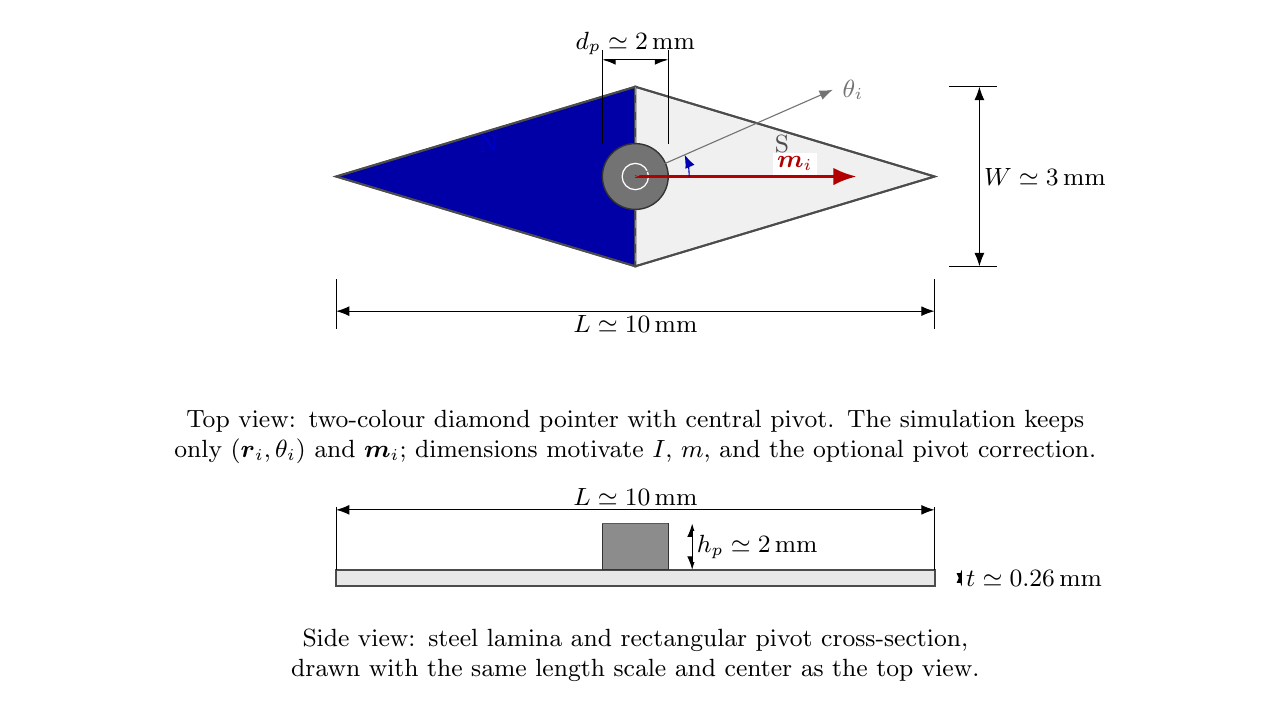
\begin{tikzpicture}[
    >=Latex,
    scale=0.76,
    every node/.style={font=\small},
    dim/.style={Latex-Latex,thin},
    lab/.style={fill=white,inner sep=1.5pt},
    steel/.style={draw=black!70,line width=0.7pt},
    north/.style={fill=blue!65!black},
    south/.style={fill=gray!12},
    pivot/.style={fill=black!55,draw=black!80,line width=0.5pt}
]
% top-view coordinates: 10 mm by 3 mm, drawn in arbitrary units
\coordinate (Ltip) at (-5,0);
\coordinate (Rtip) at (5,0);
\coordinate (Top)  at (0,1.5);
\coordinate (Bot)  at (0,-1.5);
\coordinate (C)    at (0,0);

% two magnetic halves of the diamond needle
\path[steel,north] (Ltip) -- (Top) -- (C) -- (Bot) -- cycle;
\path[steel,south] (C) -- (Top) -- (Rtip) -- (Bot) -- cycle;
\draw[steel] (Ltip) -- (Top) -- (Rtip) -- (Bot) -- cycle;
\draw[black!45,dashed] (Top) -- (Bot);

% central pivot / bearing disk
\shade[ball color=black!50] (C) circle (0.55);
\draw[pivot] (C) circle (0.55);
\draw[white,line width=0.45pt] (C) circle (0.22);

% magnetic moment and angle
\draw[->,very thick,red!70!black] (C) -- (3.7,0) node[above,pos=0.72,lab] {$\vect m_i$};
\draw[->,blue!70!black] (C) ++(0.9,0) arc[start angle=0,end angle=24,radius=0.9];
\draw[->,black!55] (C) -- ++(3.3,1.45) node[right] {$\theta_i$};
\node[blue!80!black] at (-2.45,0.55) {N};
\node[black!70] at (2.45,0.55) {S};

% length and width dimensions
\draw[dim] (-5,-2.25) -- (5,-2.25) node[midway,below,lab] {$L\simeq\SI{10}{mm}$};
\draw[thin] (-5,-1.72) -- (-5,-2.55);
\draw[thin] (5,-1.72) -- (5,-2.55);
\draw[dim] (5.75,-1.5) -- (5.75,1.5) node[midway,right,lab] {$W\simeq\SI{3}{mm}$};
\draw[thin] (5.25,-1.5) -- (6.05,-1.5);
\draw[thin] (5.25,1.5) -- (6.05,1.5);

% pivot diameter callout
\draw[dim] (-0.55,1.95) -- (0.55,1.95) node[midway,above,lab] {$d_p\simeq\SI{2}{mm}$};
\draw[thin] (-0.55,0.55) -- (-0.55,2.12);
\draw[thin] (0.55,0.55) -- (0.55,2.12);

% compact model-reduction note, placed below the top view to avoid overlap
\node[align=center,font=\small,text width=15.2cm] at (0,-4.35)
{Top view: two-colour diamond pointer with central pivot. The simulation keeps only $(\vect r_i,\theta_i)$ and $\vect m_i$; dimensions motivate $I$, $m$, and the optional pivot correction.};

% side-view inset: same horizontal scale and center as the top view
\begin{scope}[shift={(0,-6.85)}]
  \draw[steel,fill=gray!18] (-5,0) rectangle (5,0.28);
  \draw[thin] (-5,0.28) -- (-5,1.32);
  \draw[thin] (5,0.28) -- (5,1.32);
  \draw[dim] (-5,1.28) -- (5,1.28) node[midway,above,lab] {$L\simeq\SI{10}{mm}$};
  \draw[pivot,fill=black!45] (-0.55,0.28) rectangle (0.55,1.05);
  \draw[black!65,line width=0.35pt] (-0.55,1.05) -- (0.55,1.05);
  \draw[dim] (5.45,0) -- (5.45,0.28) node[midway,right,lab] {$t\simeq\SI{0.26}{mm}$};
  \draw[dim] (0.95,0.28) -- (0.95,1.05) node[midway,right,lab] {$h_p\simeq\SI{2}{mm}$};
  \node[align=center,font=\small,text width=15.2cm] at (0,-1.15) {Side view: steel lamina and rectangular pivot cross-section, drawn with the same length scale and center as the top view.};
\end{scope}
\end{tikzpicture}
\caption{Idealized geometry of the compass needle used by \code{compass.py}, based on the uploaded photographs. The actual dynamics keeps only the pivot position and angle, but the dimensions of the lamina and pivot are used to motivate $I$, $m$, and the optional pivot correction.}
\label{fig:needle_geometry}
\end{figure}



The same physical needle is then replicated on one of the lattice geometries used by the simulator. Figures~\ref{fig:square_geometry}--\ref{fig:honeycomb_geometry} show the default clean geometries exported by the code. The three panels should be read as geometry definitions rather than as simulation snapshots: every marker is a fixed pivot position, and the coloured diamond at that point represents the initial angular state of the needle. The relevant common length scale is the nearest-neighbour spacing $r_{\rm nn}$, controlled by the circumscribed radius $R$ of the needle cell; in the default construction $r_{\rm nn}\simeq2R$ for all geometries. This common spacing is essential because it makes the dipolar reference field, natural frequency, and quality factor comparable across square, triangular, and honeycomb arrays.

\begin{figure}[htbp]
\centering
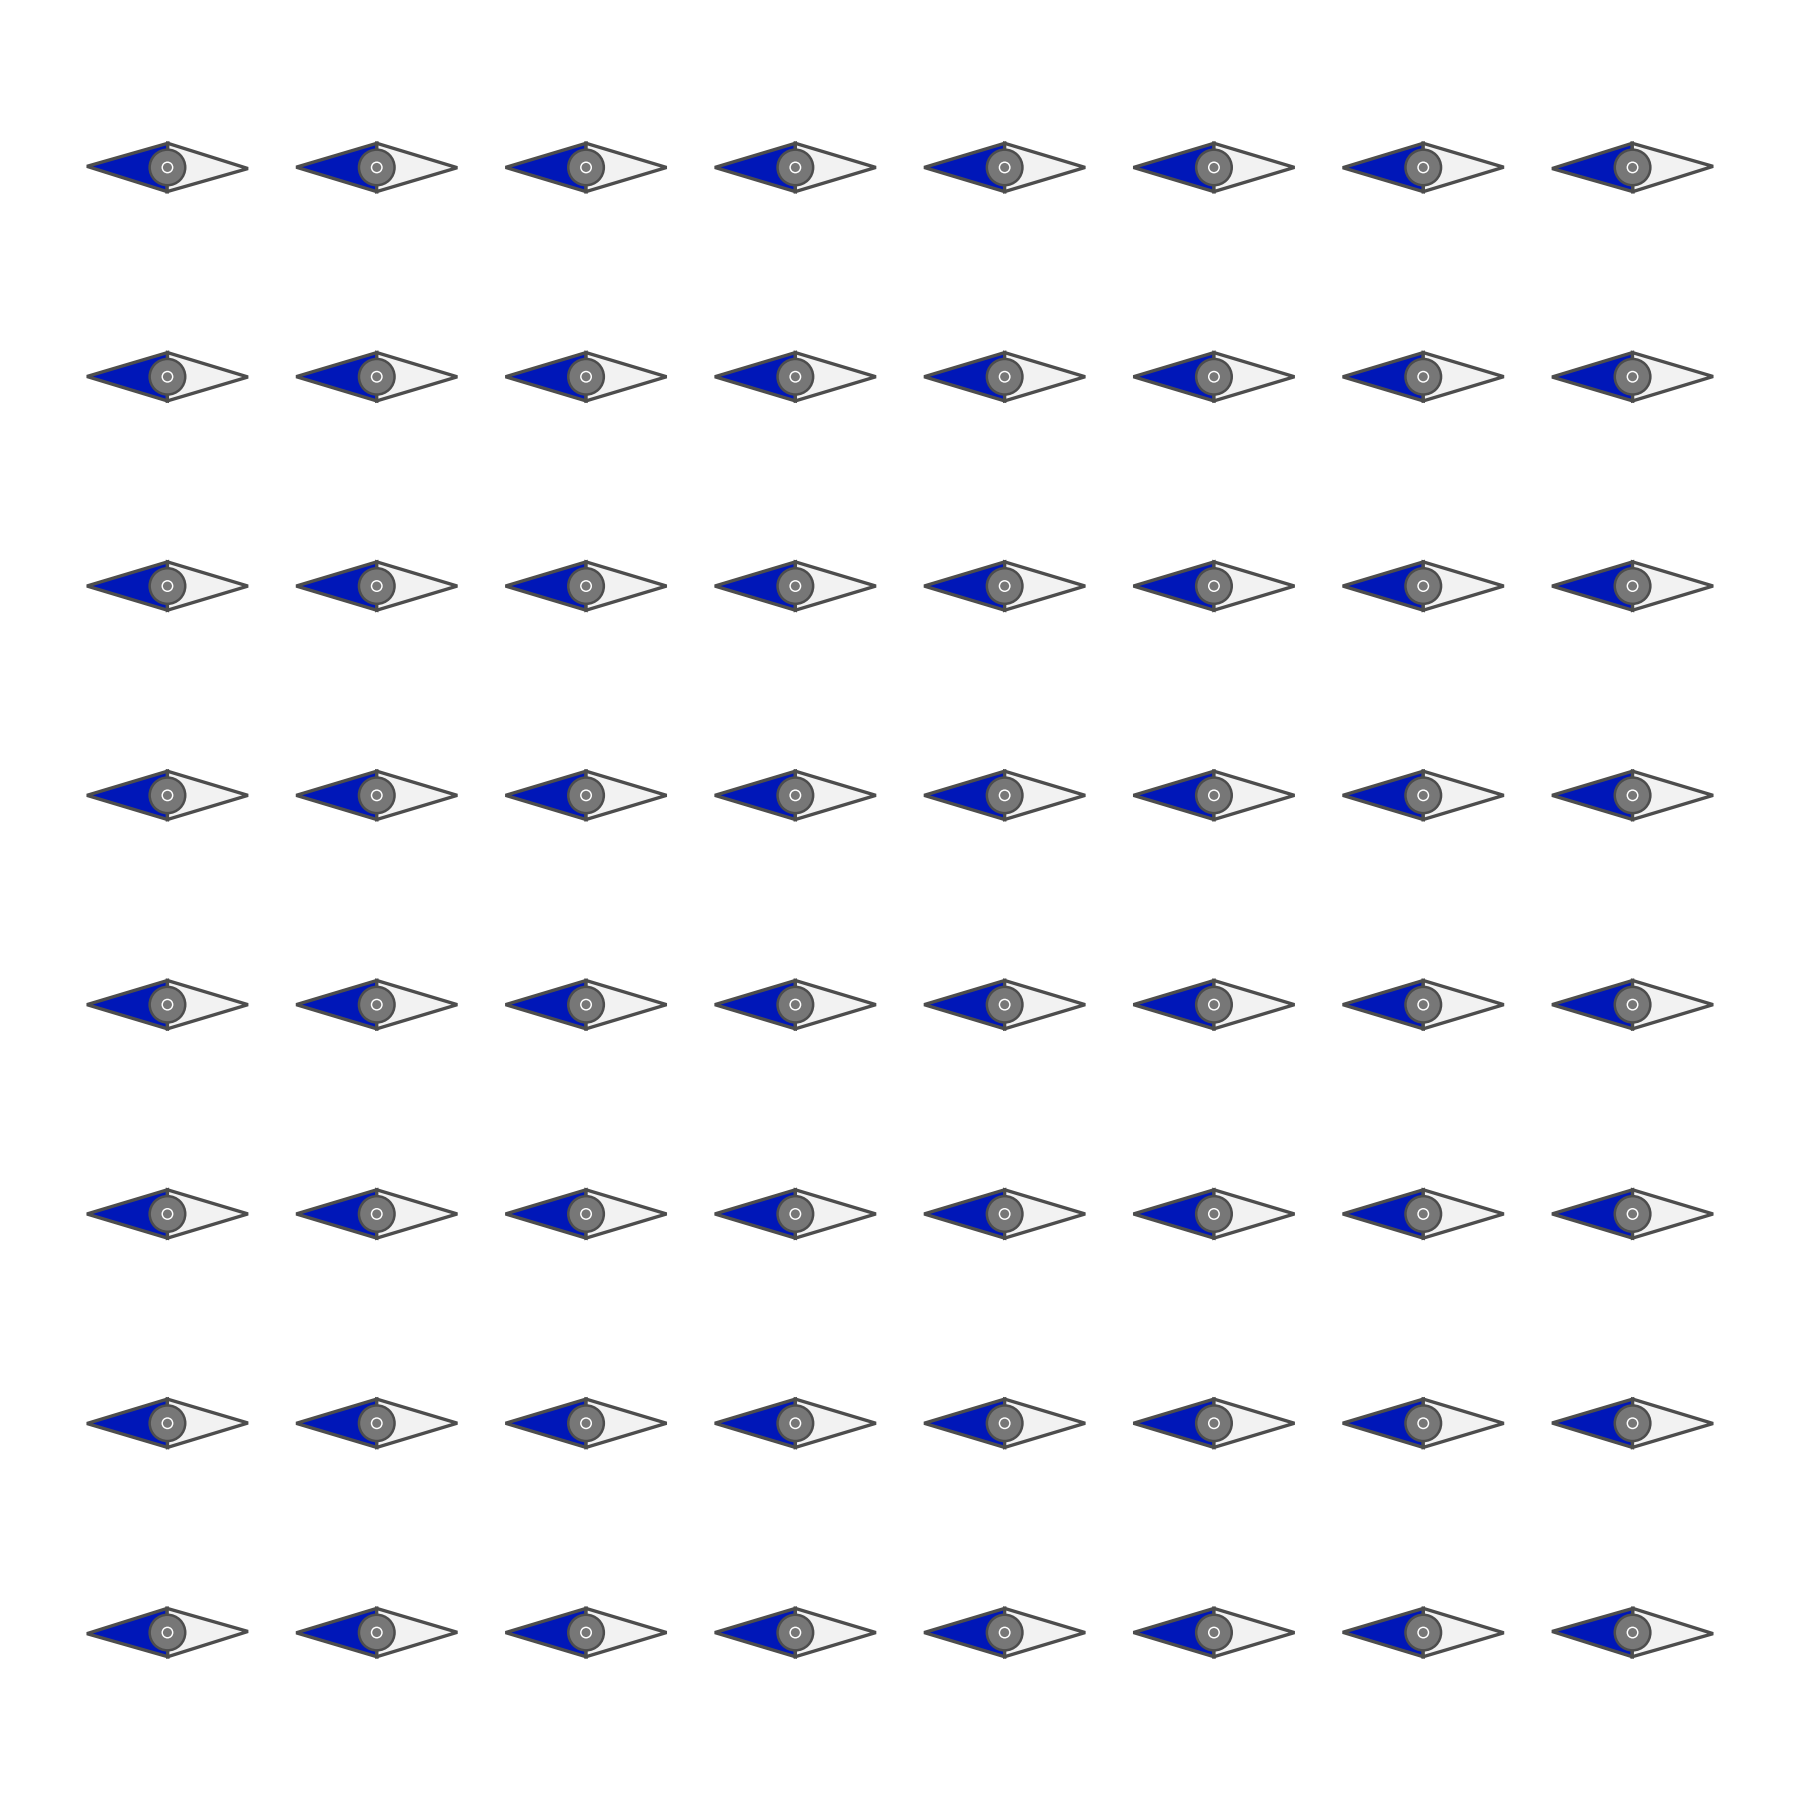
\includegraphics[width=0.62\textwidth,height=0.42\textheight,keepaspectratio]{figs/square_default_geometry_clean_colored.png}
\caption{Square-lattice geometry used by \code{compass.py}. Pivots lie on a rectangular grid with four nearest neighbours in the bulk. This is the least frustrated of the three default geometries and provides the natural baseline for interpreting domains, hysteresis loops, and avalanche activity. Because the principal lattice directions are orthogonal, field sweeps along $x$ or $y$ have a simple relation to rows and columns of needles.}
\label{fig:square_geometry}
\end{figure}

\begin{figure}[htbp]
\centering
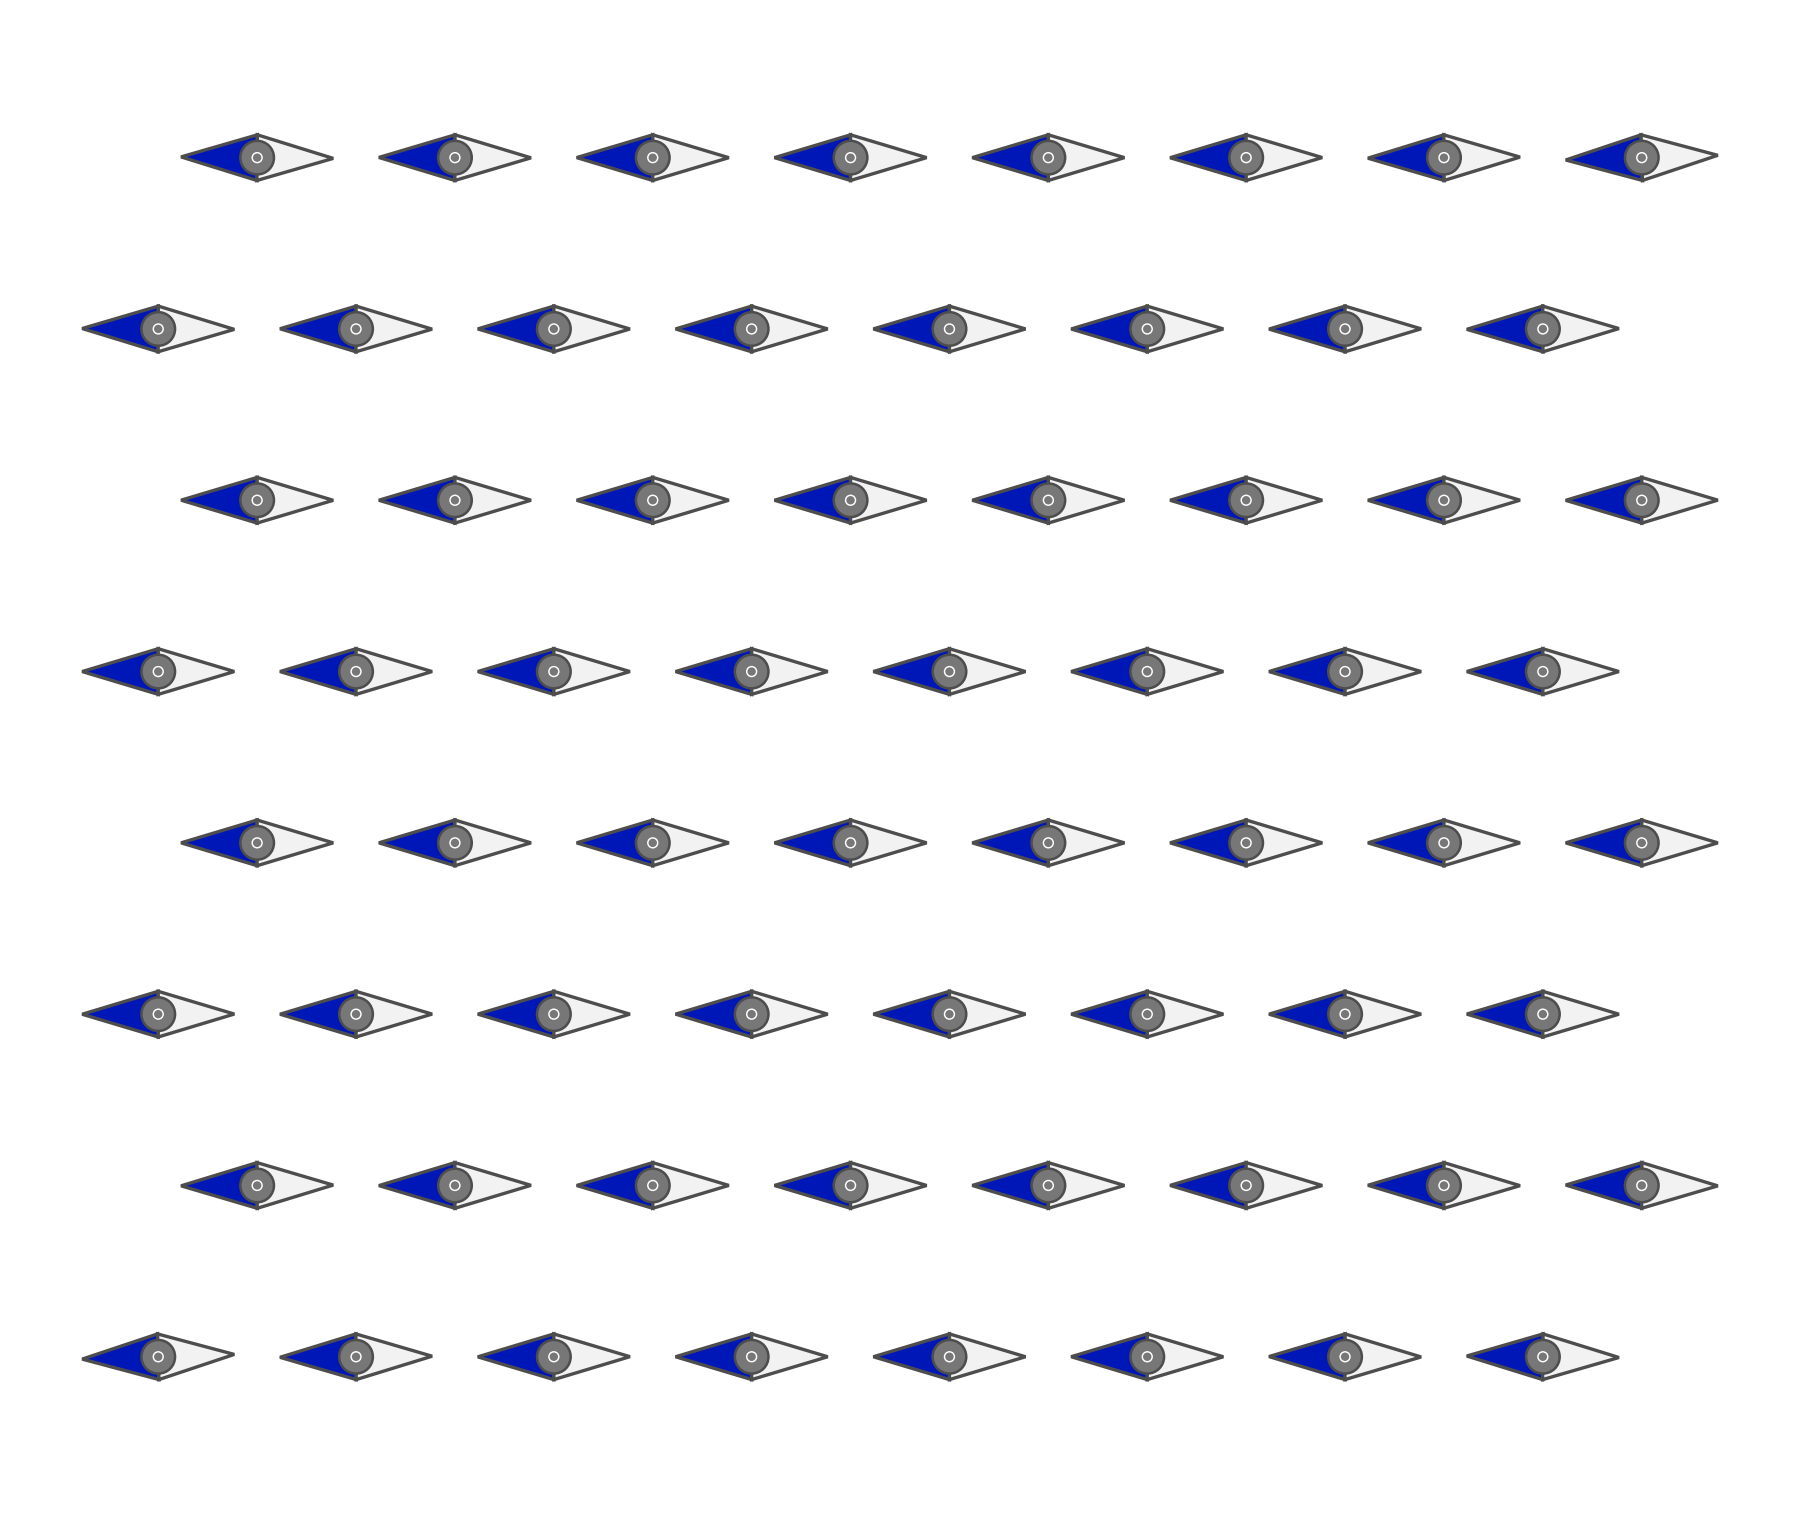
\includegraphics[width=0.62\textwidth,height=0.42\textheight,keepaspectratio]{figs/triangular_default_geometry_clean_colored.png}
\caption{Triangular-lattice geometry. Each bulk pivot has six nearest neighbours, giving the highest local coordination among the default arrays. The equilateral triangular connectivity introduces strong geometric competition for dipolar alignment, so this geometry is expected to be especially sensitive to frustration, overshoot, and damping-controlled pathway selection. It is therefore a key test case for distinguishing purely static dipolar effects from genuinely dynamical inertial effects.}
\label{fig:triangular_geometry}
\end{figure}

\begin{figure}[htbp]
\centering
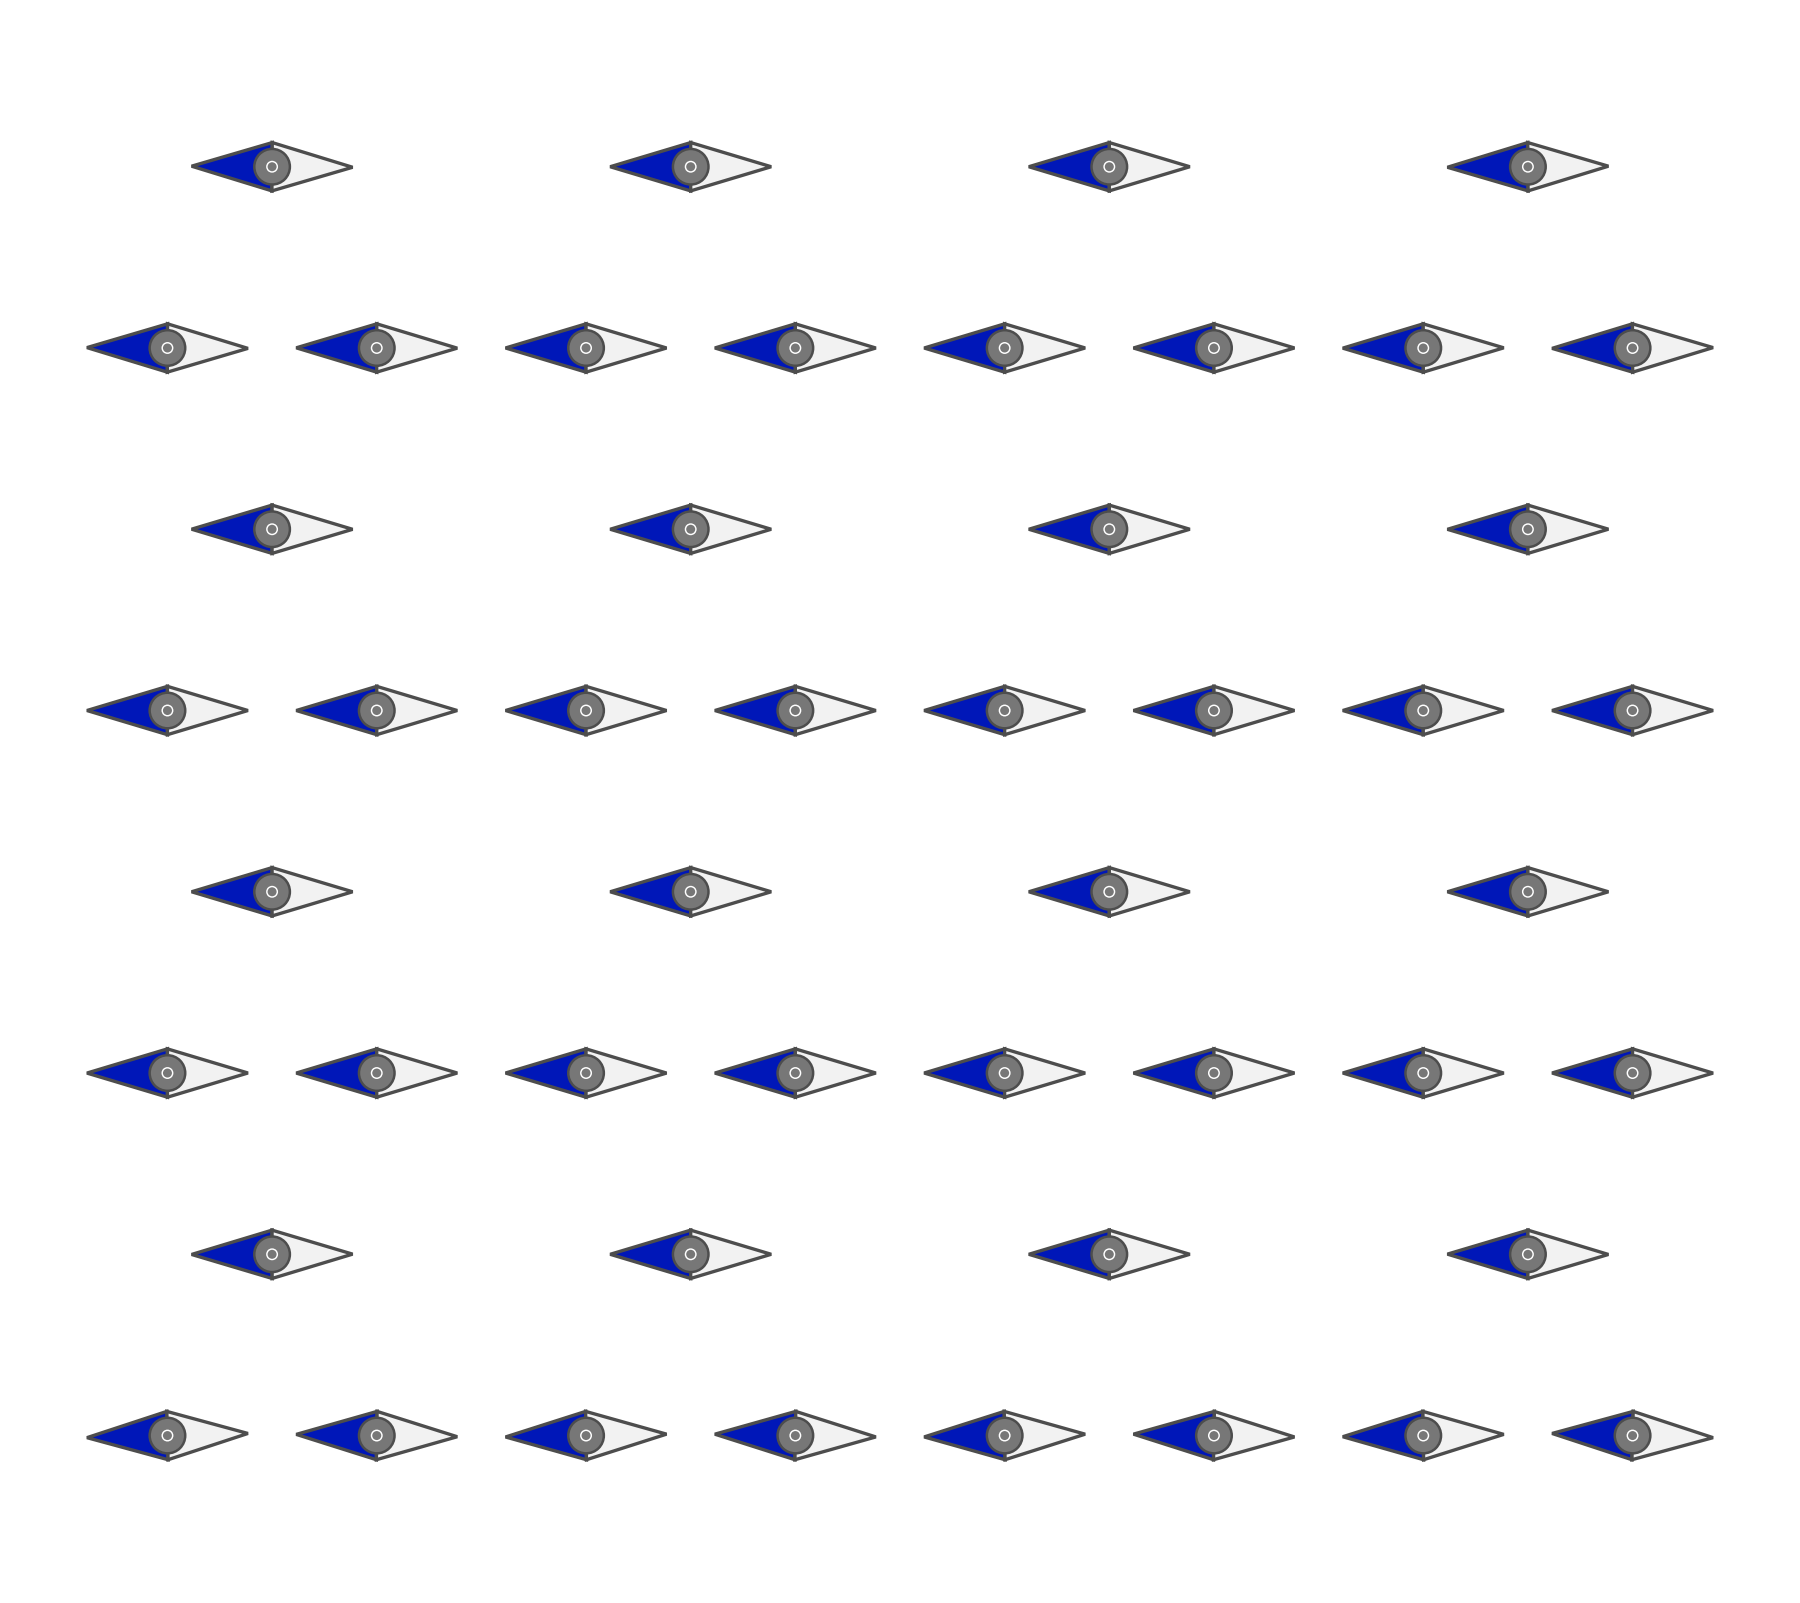
\includegraphics[width=0.62\textwidth,height=0.42\textheight,keepaspectratio]{figs/honeycomb_default_geometry_clean_colored.png}
\caption{Honeycomb-lattice geometry. The honeycomb array can be viewed as a triangular construction with systematic removal of sites, producing hexagonal voids and three nearest neighbours per bulk pivot. This lower coordination changes both the available domain-wall paths and the local reversal constraints. It also gives a geometry closer in spirit to artificial-spin-ice networks, while retaining the continuous-angle compass-needle dynamics of the present model.}
\label{fig:honeycomb_geometry}
\end{figure}

Together, these three geometries define the structural axis of the proposed research programme. The square lattice is the ordered reference case; the triangular lattice maximizes local coordination and frustration; and the honeycomb lattice reduces coordination while introducing extended hexagonal motifs. Comparing them at fixed $R$, magnetic moment $m$, inertia $I$, damping $b$, and field protocol is what allows the project to ask whether observed differences in hysteresis, avalanches, or relaxation are caused by geometry rather than by a change of physical units or numerical scale.

\subsection{Degrees of freedom}

Each needle $i$ is represented by a point magnetic dipole of fixed magnitude $m$, fixed center position $\vect r_i=(x_i,y_i)$, and one angular degree of freedom $\theta_i(t)$ in the plane. The magnetic moment is
\begin{equation}
\vect m_i = m(\cos\theta_i,\sin\theta_i,0).
\end{equation}
The model is therefore continuous-angle and inertial. It is not an Ising model, not a macrospin LLG model, and not a kinetic Monte Carlo threshold model. This is a limitation for direct comparison with nanomagnetic islands, but it is also the reason the simulator can isolate damping and overshoot.

\subsection{Dipolar field and torque}

The dipolar field at needle $i$ due to needle $j$ is
\begin{equation}
\vect B_j(\vect r_i)=\frac{\mu_0}{4\pi}\left[
\frac{3(\vect m_j\cdot \hat{\vect r}_{ij})\hat{\vect r}_{ij}-\vect m_j}{r_{ij}^3}
\right],
\qquad
\vect r_{ij}=\vect r_i-\vect r_j.
\end{equation}
The total field is the sum of all retained dipolar contributions plus the external field,
\begin{equation}
\vect B_i=\sum_{j\ne i}\vect B_j(\vect r_i)+\vect B_{\rm ext}(t).
\end{equation}
The torque about the pivot is
\begin{equation}
\tau_i = (\vect m_i\times \vect B_i)_z.
\end{equation}

\subsection{Newtonian rotational dynamics}

The equation of motion is
\begin{equation}
I\ddot\theta_i = \tau_i^{\rm dip}+\tau_i^{\rm ext}-b_i\dot\theta_i,
\label{eq:eom}
\end{equation}
where $I$ is the moment of inertia and $b_i$ is the viscous damping coefficient. The code allows uniform damping or a small random per-needle damping variation,
\begin{equation}
b_i=b\,[1+\eta_i], \qquad \eta_i\in[-\delta_b,\delta_b].
\end{equation}
This disorder is deliberately weak in the recommended campaigns. Its purpose is to break artificial degeneracies, not to dominate the physics.

The natural reference frequency is defined from a reference nearest-neighbour dipolar field,
\begin{equation}
B_{\rm ref}=\frac{\mu_0}{4\pi}\frac{2m}{r_{\rm nn}^3},
\qquad
\omega_0=\sqrt{\frac{mB_{\rm eff}}{I}},
\qquad
B_{\rm eff}=\max(B_{\rm ref},B_{\rm ext}).
\end{equation}
The quality factor is
\begin{equation}
Q=\frac{\omega_0 I}{b}.
\end{equation}
For $Q\ll 1$ the dynamics is overdamped and relaxation is slow and monotonic. For $Q\gg1$ the needles overshoot and may trigger chain-reaction switching. The regime near $Q\sim 1$ is expected to be the most sensitive because inertial memory and damping compete on comparable timescales.

\subsection{Cutoff and boundary conditions}

A critical correction in \code{compass.py} is the explicit separation between a physical cutoff in metres and a cutoff in nearest-neighbour shells:
\begin{equation}
r_{\rm cut} = c_{\rm shell} r_{\rm nn},
\end{equation}
unless the user explicitly supplies \code{--cutoff\_m}. This avoids the ambiguity present in earlier scripts, where ``3.5'' could be interpreted either as metres or as $3.5r_{\rm nn}$ depending on context.

Boundary conditions are also explicit. Free boundaries are physically meaningful for finite compass arrays and for edge nucleation. Periodic boundary conditions are useful for separating bulk behavior from sample-shape effects, but in a long-range anisotropic dipolar system they should be treated as a modelling choice, not as an automatic improvement. Every serious result should eventually be checked at least once with and without PBC.

% ======================================================================
\section{Research branch: \code{compass.py} V2.0.2}
\label{sec:compassv2}
% ======================================================================

\subsection{Reason for creating a V2 branch}

The original \code{compass.py} was strong as a visual simulator and increasingly capable as a campaign engine. However, the code still carried legacy assumptions inherited from visualization: the main scalar order parameter was $S=|\langle e^{i\theta}\rangle|$, the CSV activity column was ambiguous for avalanche analysis, energy was not logged, and the cutoff convention was not sufficiently explicit. These issues are acceptable for demonstration but not for a research claim about avalanche statistics and damping-dependent reversal.

\code{compass.py} was created as a research-oriented branch. It is not intended to replace every animation feature of \code{compass.py}; instead it prioritizes reproducibility, numerical clarity, efficient sweeps, and rich time-series output.

\subsection{New observables}

The V2 output is designed so that analysis does not need to reconstruct physics from only $M(t)$ and $B(t)$. The standard CSV now includes the following classes of observables:

\begin{longtable}{@{}p{4.2cm}p{10.6cm}@{}}
\caption{Main research observables in \code{compass.py}.}\label{tab:v2obs}\\
\toprule
\textbf{Observable} & \textbf{Purpose}\\
\midrule
\endfirsthead
\toprule
\textbf{Observable} & \textbf{Purpose}\\
\midrule
\endhead
\bottomrule
\endfoot
$M_x$, $M_y$ & Mean polar magnetization components. Their vector magnitude is $S_1$ in the current CSV, so no separate $M_{\rm abs}$ column is written.\\
$M_{\rm proj}$ & Magnetization projected along the applied-field direction. This is the relevant scalar for hysteresis loops.\\
$S_1=|\langle e^{i\theta}\rangle|$ & Polar order parameter. Sensitive to net alignment, but can miss antiparallel line order.\\
$S_2=|\langle e^{2i\theta}\rangle|$ & Nematic/director order parameter. Detects axis selection even when opposite directions cancel. Essential for compass-lattice director memory.\\
$\theta_{\rm dir}$ & Director angle, defined modulo $\pi$. Used for pulse-memory and line-order studies.\\
$q_{\rm axis}$ & Square-lattice-inspired axis-population imbalance. Useful for comparison with compass-lattice line formation.\\
\code{flip\_field} & Number of sign reversals relative to the field axis between logged states. A discrete activity channel for field-driven avalanches.\\
\code{flip\_angle} & Number of needles whose angular increment exceeds a threshold. A field-independent activity channel useful near zero field and in relaxation.\\
$E_{\rm dip}$, $E_{\rm ext}$, $K_{\rm rot}$, $E_{\rm total}$ & Energy ledger. Needed to interpret relaxation pathways, dissipation, and numerical stability.\\
$\omega_{\rm rms}$, $\omega_{\rm max}$ & Dynamical activity indicators. Useful to identify residual oscillations and compare damping regimes.\\
\end{longtable}

The addition of $S_2$ is particularly important. A square compass array may develop line or director order while the net magnetization remains small. A simulator that logs only $S_1$ can therefore misidentify an ordered state as disordered.

\subsection{Field protocols}

The current V2 protocol set is:
\begin{itemize}[leftmargin=*]
\item \code{static}: constant field.
\item \code{hysteresis}: five-segment loop $0\to +B_{\max}\to0\to-B_{\max}\to0\to+B_{\max}$.
\item \code{forc}: repeated saturation, descent to reversal field $B_r$, and return to positive saturation.
\item \code{sine}: sinusoidal applied field.
\item \code{step\_up}/\code{step\_pos}: zero field followed by field-on relaxation.
\item \code{step\_down}/\code{step\_neg}: field initially on, then removed.
\item \code{pulse}: delayed finite-duration field pulse followed by zero-field relaxation.
\item \code{demag\_rot}: rotating field with decreasing amplitude.
\item \code{demag\_linear}: linearly decreasing field along a fixed direction.
\end{itemize}

The scientific distinction among these modes is important. Hysteresis measures reversal under continuous forcing. FORC probes history-dependent partial reversal. Step and pulse protocols probe relaxation and memory after a controlled perturbation. Demagnetization protocols prepare initial states and should not be confused with the measurement itself.


\subsection{Output files}

Each V2.0.2 run writes a tagged directory tree under \code{--out\_dir}. The current implementation creates four subdirectories:
\begin{itemize}[leftmargin=*]
\item \code{data/}: CSV time series, written as \code{data/<tag>.csv};
\item \code{meta/}: JSON metadata, written as \code{meta/<tag>.json};
\item \code{states/}: compressed initial and final state files, \code{states/<tag>\_initial.npz} and \code{states/<tag>\_final.npz};
\item \code{images/}: automatic lattice figures, \code{images/<tag>\_initial\_lattice.png}, \code{images/<tag>\_final\_lattice.png}, and \code{images/<tag>\_initial\_final.png}.
\end{itemize}

The initial state is saved before time integration, after lattice generation, random angular initialization, physical-parameter derivation, protocol construction, tensor precomputation, and metadata assembly. The final state is saved after the full integration and contains the final angles and angular velocities. Both state files contain \code{xs}, \code{ys}, \code{theta}, \code{omega}, \code{r\_nn}, and a serialized \code{metadata\_json} field. This design makes the automatic figures reproducible without re-running the simulation.

The metadata records the program name, version, \code{source\_file\_timestamp}, \code{created\_unix\_time}, \code{created\_datetime\_utc}, \code{created\_datetime\_local}, the effective configuration, derived quantities such as $K$, $r_{\rm nn}$, $B_{\rm ref}$, $B_{\rm eff}$, $\omega_0$, $T_0$, $\Delta t$, $Q$, cutoff policy, tensor memory, numerical dtype, final domain statistics, and runtime. The CSV alone is therefore not treated as a complete scientific record; interpretation also requires the JSON metadata and the state snapshots.

The \code{--make\_plot} option is now separate from lattice visualization. Lattice PNGs are generated automatically for every run, while \code{--make\_plot} adds diagnostic time-series plots based on the CSV.

\subsection{Efficiency design}


The main computational cost is the dipolar field, which scales as $K^2$ for $K$ needles. Since needle positions are fixed, V2 uses a precomputed interaction tensor when memory allows. The field is then obtained from matrix-vector products rather than rebuilding all pair separations at every time step. This is efficient on CPU through BLAS and can also benefit from GPU acceleration for sufficiently large arrays.

The code also provides \code{--float32} for exploratory GPU or memory-limited scans. Final publication-quality results should remain in double precision unless a documented convergence test shows that single precision gives indistinguishable observables.

% ======================================================================
\section{Literature gaps and study cases}
\label{sec:gaps}
% ======================================================================

\subsection{Compass needles: what is already known}

The compass-needle literature already established the value of macroscopic dipolar analogues. Olive and Molho studied a square $22\times22$ lattice, random-field excitation, line length, director selection, and a mapping between a dissipative experimental system and Monte Carlo thermodynamics~\cite{olive1998}. Novak and Sinnecker showed that hysteresis and magnetization processes in compass-needle arrays depend strongly on number and arrangement of needles, through magnetostatic coupling~\cite{novak2004}. These works justify the model, but they do not answer the present dynamical question because they did not sweep Newtonian damping as a controlled parameter in long-range simulated arrays.

\subsection{Artificial spin ice: why it is relevant but not identical}

Artificial spin ice consists of coupled nanomagnets whose geometry creates frustration, domains, monopole-like excitations, memory, and programmable dynamics~\cite{nisoli2013,skjaervoe2020}. Recent work on clocked dynamics shows that field protocols can control domain growth and reversal in artificial spin ice, but also emphasizes how difficult it is to control avalanche-like activity with ordinary field sweeps~\cite{jensen2024}. The compass model is not a nanolithographic ASI model in the strict sense, because it lacks shape-anisotropy switching astroids and Ising-like barriers. Nevertheless, it is a clean platform for asking which dynamic features arise already from long-range dipolar coupling plus inertia.

\subsection{Avalanches and magnetic charges}

Theoretical work on artificial spin ice has described reversal in terms of domain walls and effective magnetic charges, with positive feedback leading to avalanches~\cite{mellado2010}. The compass model should not claim true monopole dynamics unless a charge-mapping observable is explicitly defined. However, it can test a related and more general question: under what dynamical conditions does local dipolar reversal amplify into a correlated switching cascade?

\subsection{FORC in correlated systems}

FORC diagrams are often used to infer switching and interaction-field distributions~\cite{pike1999,roberts2000}. However, in correlated systems the interpretation of FORC diagrams as intrinsic switching-field distributions can fail~\cite{ruta2017}. This is an excellent opportunity for \code{compass.py}: if a system with known identical dipoles and no intrinsic switching-field dispersion produces broad FORC structure, then that structure must be collective and history-dependent. FORC then becomes a diagnostic of correlated dynamics, not a direct inversion of particle thresholds.

\subsection{Relaxation pathways and memory}

Recent ASI studies show that relaxation pathways and domain morphology depend on local torques, switching barriers, and path selection, not only on equilibrium energetics~\cite{menniti2025}. Other work connects ASI to reservoir computing and memory, where dipolar interactions affect echo-state behavior and memory capacity~\cite{taniguchi2025}. The compass model can contribute here by measuring relaxation after step and pulse protocols in a system where inertia and damping are explicit.

% ======================================================================
\section{Proposed research studies}
\label{sec:studies}
% ======================================================================

\subsection{Study 1: damping-controlled hysteresis and avalanches}

\textbf{Question.} Does $Q$ change hysteresis shape and avalanche statistics in square, triangular, and honeycomb dipolar lattices?

\textbf{Protocol.} Use \code{field\_mode hysteresis}. Sweep $Q$ logarithmically from deep overdamped to strongly underdamped. Use multiple seeds and weak damping disorder.

\textbf{Observables.} Loop area, coercive field, remanence, $P(s)$ from \code{flip\_field} and \code{flip\_angle}, waiting times, $M(t)$ autocorrelation, $E_{\rm total}(t)$, and final domain/director metrics.

\textbf{Critical analysis.} Do not rely on only $dM/dB$ thresholding. Use the native flip counters as primary activity measures. Fit power laws only after checking tail size, cutoff stability, and alternatives such as log-normal distributions. Report when statistics are insufficient.

\subsection{Study 2: FORC fingerprints of correlated reversal}

\textbf{Question.} Can correlated dipolar dynamics produce FORC structures even in an array of identical needles with no intrinsic switching-field distribution?

\textbf{Protocol.} Use \code{field\_mode forc}. Run selected values $Q=0.05,0.3,1.0,3.0,15,30$ for square and triangular arrays first. Add honeycomb only after FORC processing is stable.

\textbf{Observables.} FORC branch families, local slopes, irreversible activity along reversal curves, energy loss along minor loops, and apparent interaction-field width.

\textbf{Critical analysis.} Treat the FORC diagram as a dynamic fingerprint. Avoid interpreting the FORC distribution as a Preisach distribution unless return-point memory and weak-correlation assumptions are explicitly checked.

\subsection{Study 3: step-up and step-down relaxation}

\textbf{Question.} How does an initially disordered or saturated dipolar array relax after a sudden field change, and how does the relaxation time depend on $Q$?

\textbf{Protocol.} Use \code{step\_up} and \code{step\_down}. In \code{step\_up}, start from noisy angles and switch on a field after a delay. In \code{step\_down}, initialize or drive into a field-biased state and remove the field.

\textbf{Observables.} Relaxation time, $S_1(t)$, $S_2(t)$, $\theta_{\rm dir}(t)$, flip activity, kinetic energy decay, and residual domain structure.

\textbf{Hypothesis.} Overdamped arrays should show slower but more monotonic relaxation. Underdamped arrays may show faster initial alignment but longer oscillatory tails and more secondary avalanches.

\subsection{Study 4: pulse-written metastability and director memory}

\textbf{Question.} Can a finite field pulse write a metastable domain or director state whose memory depends on $Q$, pulse duration, and geometry?

\textbf{Protocol.} Use \code{pulse}. Sweep pulse duration in units of $T_0$ and amplitude in units of $B_{\rm ref}$. For each run, allow a zero-field relaxation tail long enough to measure the final director and domain state.

\textbf{Observables.} Correlation between pulse direction and final director,
\begin{equation}
C_{\rm mem}=\left\langle \cos 2(\theta_{\rm dir}^{\rm final}-\phi_{\rm pulse})\right\rangle,
\end{equation}
final $S_2$, domain-size distribution, and post-pulse activity.

\textbf{Critical analysis.} This study is close in spirit to clocked ASI dynamics, but should not be described as astroid clocking. The compass system has no switching astroids. It tests pulse-induced memory in a continuous dipolar array.

\subsection{Study 5: finite size, cutoff, and boundary conditions}

\textbf{Question.} Which conclusions survive changes in system size, cutoff, and boundary condition?

\textbf{Protocol.} Repeat selected $Q$ values for $N=20,30,40,50$ and cutoffs $2.5r_{\rm nn}$, $3.5r_{\rm nn}$, $5r_{\rm nn}$, with and without PBC.

\textbf{Critical analysis.} This is not optional. Dipolar systems are sensitive to sample shape. A result based only on one finite free-boundary array is suggestive but not conclusive.

% ======================================================================
\section{Recommended campaigns and commands}
\label{sec:commands}
% ======================================================================

\subsection{Single-run smoke test}

Before any campaign, run a short test and inspect the CSV and JSON:

\begin{lstlisting}[style=bashstyle]
python3 compass.py \
  --out_dir ~/results/compassV02_smoke \
  --tag smoke_square_hyst \
  --geometry square \
  --N 12 --M 12 \
  --field_mode hysteresis \
  --B_max_factor 8.0 \
  --t_sim 1.5 \
  --cutoff_shells 3.5 \
  --dt_factor 0.04 \
  --log_every 5 \
  --seed 12345 \
  --verbose \
  --make_plot
\end{lstlisting}

After this command the run should contain not only \code{data/}, \code{meta/}, and \code{states/}, but also \code{images/}. In particular, the smoke test should create \code{smoke\_square\_hyst\_initial\_lattice.png}, \code{smoke\_square\_hyst\_final\_lattice.png}, and \code{smoke\_square\_hyst\_initial\_final.png} in the \code{images/} subdirectory. These figures are produced automatically; \code{--make\_plot} only requests the additional CSV diagnostic plots.

\subsection{Main hysteresis campaign using \code{compass.py}}

The following command is for one representative run. A wrapper should loop over geometry, seed, and damping or directly compute damping values from desired $Q$.

\begin{lstlisting}[style=bashstyle]
python3 compass.py \
  --out_dir ~/results/law3m_2026_v02/main_hysteresis \
  --tag square_Qscan_seed000 \
  --geometry square \
  --N 36 --M 36 \
  --field_mode hysteresis \
  --B_max_factor 8.0 \
  --t_sim 8.0 \
  --cutoff_shells 3.5 \
  --damping 5e-8 \
  --damping_noise 0.05 \
  --dt_factor 0.035 \
  --log_every 10 \
  --seed 1000 \
  --verbose
\end{lstlisting}

\subsection{FORC subset}

\begin{lstlisting}[style=bashstyle]
python3 compass.py \
  --out_dir ~/results/law3m_2026_v02/forc_subset \
  --tag square_Q1_forc_seed000 \
  --geometry square \
  --N 30 --M 30 \
  --field_mode forc \
  --B_max_factor 8.0 \
  --forc_n_curves 41 \
  --forc_Br_min -0.002 \
  --forc_rate 2.0e-4 \
  --cutoff_shells 3.5 \
  --damping 1.0e-6 \
  --damping_noise 0.03 \
  --dt_factor 0.035 \
  --log_every 5 \
  --seed 2000 \
  --verbose
\end{lstlisting}

The numerical value of \code{--forc\_Br\_min} should normally be derived from the actual $B_{\max}$ of the run. The explicit value shown above is only a template.

\subsection{Step-down relaxation}

\begin{lstlisting}[style=bashstyle]
python3 compass.py \
  --out_dir ~/results/law3m_2026_v02/step_relax \
  --tag triangular_stepdown_Q3_seed000 \
  --geometry triangular \
  --N 36 --M 36 \
  --field_mode step_down \
  --B_max_factor 8.0 \
  --field_delay 2.0 \
  --t_sim 10.0 \
  --cutoff_shells 3.5 \
  --damping 5e-7 \
  --damping_noise 0.05 \
  --dt_factor 0.035 \
  --log_every 10 \
  --seed 3000 \
  --verbose
\end{lstlisting}

\subsection{Pulse-memory run}

\begin{lstlisting}[style=bashstyle]
python3 compass.py \
  --out_dir ~/results/law3m_2026_v02/pulse_memory \
  --tag square_pulse_phi45_seed000 \
  --geometry square \
  --N 36 --M 36 \
  --field_mode pulse \
  --B_max_factor 6.0 \
  --phi_ext_deg 45 \
  --field_delay 1.0 \
  --t_pulse 1.5 \
  --t_sim 10.0 \
  --cutoff_shells 3.5 \
  --damping 5e-7 \
  --damping_noise 0.05 \
  --dt_factor 0.035 \
  --log_every 10 \
  --seed 4000 \
  --verbose
\end{lstlisting}

\subsection{Status of \code{damping\_sweepV02.py}}

The older \code{damping\_sweepV02.py} remains useful as a campaign pattern: it implements parallel execution, incremental manifest writing, and resume. However, before it is used for the definitive V2.0.2 campaign, it should be updated to call \code{compass.py} or import its functions. Otherwise it will not benefit from timestamped metadata, automatic initial/final state snapshots, automatic lattice PNG generation, unambiguous cutoff handling, energy output, and native avalanche counters. The new wrapper should preserve the good features of V02: worker sandboxing, \code{--resume}, and a consolidated manifest.

% ======================================================================
\section{Validation plan}
\label{sec:validation}
% ======================================================================

No result should be interpreted physically until the following checks have been performed and recorded.

\begin{enumerate}[leftmargin=*]
\item \textbf{Torque validation.} Compare tensor torques with direct pairwise torques for small arrays, with and without PBC.
\item \textbf{Energy consistency.} During static zero-damping tests, verify that total mechanical plus dipolar plus external energy is conserved to the expected numerical tolerance. With damping, verify monotonic kinetic-energy decay after the field is removed, apart from dipolar energy exchange.
\item \textbf{Time-step convergence.} Repeat representative cases with \code{dt\_factor} values 0.05, 0.035, 0.025, and 0.015. Avalanche exponents and loop metrics should not change beyond statistical uncertainty.
\item \textbf{Cutoff convergence.} Repeat representative cases at $2.5r_{\rm nn}$, $3.5r_{\rm nn}$, and $5r_{\rm nn}$. If conclusions depend strongly on cutoff, this must be part of the physics discussion.
\item \textbf{Finite-size convergence.} Repeat at $N=20,30,40$ for at least three $Q$ values. Check whether avalanche cutoffs scale with system size and whether fitted exponents remain stable.
\item \textbf{Boundary sensitivity.} Compare free and periodic boundaries. In dipolar systems, boundary effects are not a numerical nuisance; they can be physical.
\item \textbf{CPU/GPU equivalence.} If \code{--use\_gpu} is used, compare selected runs against CPU double precision. If \code{--float32} is used, label results exploratory until convergence is proven.
\item \textbf{Avalanche definition robustness.} Compare \code{flip\_field}, \code{flip\_angle}, and derivative-based activity. A result seen by only one arbitrary threshold is weak.
\item \textbf{FORC sanity.} Verify that FORC curves are sampled at constant sweep rate if the objective is to compare reversal branches. Variable sweep rates can create artificial dynamic differences.
\end{enumerate}

% ======================================================================
\section{Data analysis strategy}
\label{sec:analysis}
% ======================================================================

The analysis should be organized around data products, not only around plots. For every campaign the following files should be produced:

\begin{enumerate}[leftmargin=*]
\item \code{manifest.csv}: one row per run, including geometry, seed, damping, $Q$, field protocol, cutoff, PBC flag, output paths, and code version.
\item \code{summary\_loops.csv}: loop area, coercive field, remanence, saturation quality, and numerical flags.
\item \code{summary\_avalanches.csv}: avalanche counts, size distributions, waiting times, fitted exponents, tail sizes, and model-comparison statistics.
\item \code{summary\_relaxation.csv}: relaxation times, final $S_1$, $S_2$, $q_{\rm axis}$, director angle, domain count, and mean domain size.
\item \code{summary\_energy.csv}: energy loss, kinetic-energy peaks, and energy relaxation times.
\item \code{quality\_control.csv}: warnings for insufficient avalanche statistics, time-step instability, failure to saturate, or excessively large residual kinetic energy.
\end{enumerate}

The most important methodological rule is aggregation by physical condition. Avalanche fits should aggregate seeds for each $(geometry,Q)$ condition before fitting. A single run rarely provides enough events for a reliable exponent.

% ======================================================================
\section{Laboratory chronology}
\label{sec:chronology}
% ======================================================================

\subsection{Initial phase: visual dipolar simulator}

The earliest version implemented a square array of compass needles, top-view visualization, and full dipolar interactions. The original objective was to reproduce intuitive magnetic behavior: alignment, domain-like textures, and hysteresis. This phase was valuable because it forced the model to use real SI units and real needle geometry rather than arbitrary dimensionless parameters.

\subsection{Expansion phase: field protocols and geometries}

The simulator then gained triangular and honeycomb geometries, dynamic field modes, hysteresis cycles, sine fields, pulse and step protocols, periodic boundary conditions, and CSV export. This changed the program from an animation into a numerical experiment platform.

\subsection{Campaign phase: damping sweeps}

The first campaign scripts introduced the central idea: sweep damping or $Q$ across geometries and seeds, then analyze hysteresis, avalanches, and relaxation. The pilot results suggested a systematic dependence of avalanche statistics on $Q$, but the old CSV structure was not yet ideal for a strong claim because the activity channel was not a true flip counter.

\subsection{Research-grade refactoring: \code{compass.py}}

The V2 branch addressed the methodological weaknesses identified during critical review. The main changes were:

\begin{itemize}[leftmargin=*]
\item explicit cutoff convention, with \code{--cutoff\_shells} and \code{--cutoff\_m};
\item polar, nematic, and axis-order observables;
\item native activity counters for avalanche studies;
\item energy ledger and angular-velocity diagnostics;
\item reproducible timestamped metadata, initial/final state snapshots, and automatic lattice PNGs;
\item field protocols suitable for hysteresis, FORC, step, pulse, sine, and demagnetization studies;
\item efficiency through precomputed dipolar tensors and optional GPU backend.
\end{itemize}

This is the point at which the code becomes credible as a research tool, provided the validation plan is followed.

% ======================================================================
\section{Remaining limitations and necessary future improvements}
\label{sec:limitations}
% ======================================================================

\begin{enumerate}[leftmargin=*]
\item \textbf{The model is not a nanoisland switching model.} It lacks shape-anisotropy energy barriers and Stoner-Wohlfarth astroids. Comparisons with artificial spin ice must be conceptual, not one-to-one.
\item \textbf{Thermal noise is not yet a physical Langevin bath.} The present demagnetization/noise tools are useful protocols, but a rigorous finite-temperature model would require fluctuation-dissipation-consistent stochastic torques.
\item \textbf{Domain analysis needs a dedicated V2 postprocessor.} Final-state images are not enough. Domain labels, domain-wall length, cluster anisotropy, and director persistence should be computed from saved states.
\item \textbf{FORC diagrams require a proper derivative pipeline.} FORC curves alone are not the same as FORC distributions. A smoothing and differentiation procedure, with sensitivity analysis, must be implemented.
\item \textbf{Wrapper scripts must be updated to V2.} The old \code{damping\_sweepV02.py} architecture is useful, but the production wrapper should call \code{compass.py} and use the new CSV/metadata columns.
\item \textbf{GPU mode must be benchmarked conservatively.} GPU can be faster for large single runs, but CPU multiprocessing is often more robust for many independent sweeps. Do not combine multiple worker processes with one GPU context unless explicitly engineered.
\item \textbf{Publication figures are still a separate need.} The V2 branch prioritizes data. A paper-figure script should make clean, white-background, vector or high-resolution plots with consistent labels.
\end{enumerate}

% ======================================================================
\section{Next steps}
\label{sec:next}
% ======================================================================

\begin{enumerate}[leftmargin=*]
\item Run the V2 smoke tests for square, triangular, and honeycomb lattices.
\item Create \code{damping\_sweepV03.py} or \code{compassV02\_sweep.py}, preserving V02 parallelism and resume but using V2 outputs.
\item Run a reduced V2 campaign: $N=20$, three geometries, five $Q$ values, three seeds. Confirm that the output and analysis pipeline are coherent.
\item Run the main LAW3M-scale campaign only after the reduced campaign passes validation.
\item Implement a FORC postprocessor that constructs FORC distributions and records smoothing sensitivity.
\item Implement a pulse/step postprocessor for director memory, $S_2(t)$ relaxation, and energy decay.
\item Prepare a conference figure set: $\tau(Q)$, loop area vs. $Q$, representative avalanche histograms, $S_2(t)$ after pulses, and FORC fingerprints for overdamped vs. underdamped regimes.
\item For a manuscript, frame the contribution as damping-controlled correlated reversal in a minimal long-range dipolar dynamical system. Avoid overclaiming equivalence to nanolithographic ASI.
\end{enumerate}

% ======================================================================
\section{Appendix A: \code{compass.py} command-line reference}
\label{app:cli}
% ======================================================================

\begin{longtable}{@{}p{4.4cm}p{10.4cm}@{}}
\caption{Main command-line parameters of \code{compass.py} V2.0.2.}\label{tab:cli}\\
\toprule
\textbf{Parameter} & \textbf{Meaning}\\
\midrule
\endfirsthead
\toprule
\textbf{Parameter} & \textbf{Meaning}\\
\midrule
\endhead
\bottomrule
\endfoot
\code{--geometry} & \code{square}, \code{triangular}, or \code{honeycomb}. The current honeycomb generator follows the finite hexagonal-hole convention inherited from the earlier code, and the actual nearest-neighbour distance is computed from the generated sites.\\
\code{--N}, \code{--M} & Number of rows/columns or nominal honeycomb dimensions.\\
\code{--R} & Half the centre-to-centre distance between neighbouring pivots. The default \code{R=0.0065} gives a \SI{13}{mm} nominal spacing.\\
\code{--needle\_len}, \code{--needle\_width}, \code{--needle\_thickness} & Physical dimensions of the rhombus-shaped needle blade. Defaults are \SI{10}{mm}, \SI{3}{mm}, and \SI{0.4}{mm}.\\
\code{--needle\_frac}, \code{--use\_legacy\_size\_from\_R} & Backward-compatible visualization convention. By default, physical needle dimensions are independent of lattice spacing; if legacy mode is enabled, the blade size is derived from \code{needle\_frac*2R}.\\
\code{--moment}, \code{--inertia} & Explicit overrides for magnetic moment and moment of inertia. If omitted, the code derives them from geometry and material parameters.\\
\code{--steel\_density}, \code{--steel\_Ms}, \code{--steel\_Bsat} & Material parameters for automatic physical derivation of $m$ and $I$. \code{--steel\_Bsat}, when supplied, overrides \code{--steel\_Ms}.\\
\code{--pivot\_radius}, \code{--pivot\_thickness}, \code{--pivot\_density}, \code{--pivot\_mass} & Optional pivot-hole and pivot-cylinder corrections for inertia and magnetic volume.\\
\code{--damping}, \code{--damping\_noise} & Central viscous damping and random per-needle relative damping variation.\\
\code{--t\_sim}, \code{--dt\_factor}, \code{--noise}, \code{--seed}, \code{--log\_every} & Simulation time, time-step factor $\Delta t/T_0$, initial angular noise amplitude, random seed, and CSV output cadence.\\
\code{--flip\_angle\_deg} & Threshold for the field-independent large-rotation activity counter.\\
\code{--cutoff\_shells}, \code{--cutoff\_m} & Dipolar cutoff in units of the computed nearest-neighbour distance or as an absolute length. \code{--cutoff\_m} overrides \code{--cutoff\_shells}.\\
\code{--pbc}, \code{--n\_images} & Periodic boundary conditions and number of periodic images in each direction.\\
\code{--tensor\_mem\_limit\_gb} & Memory limit for the precomputed dipolar tensor.\\
\code{--float32} & Single precision for exploratory runs. Double precision remains preferred for final results.\\
\code{--field\_mode} & \code{static}, \code{hysteresis}, \code{forc}, \code{sine}, \code{step\_up}, \code{step\_pos}, \code{step\_down}, \code{step\_neg}, \code{pulse}, \code{demag\_rot}, or \code{demag\_linear}.\\
\code{--B\_ext}, \code{--B\_max\_factor}, \code{--phi\_ext\_deg} & Applied field amplitude, automatic amplitude factor relative to $B_{\rm ref}$, and field direction.\\
\code{--field\_freq}, \code{--field\_delay}, \code{--t\_pulse} & Sinusoidal frequency and timing parameters for step and pulse protocols.\\
\code{--hyst\_spacing}, \code{--hyst\_log\_k} & Linear or logarithmic spacing for the five-segment hysteresis field schedule.\\
\code{--forc\_n\_curves}, \code{--forc\_Br\_min}, \code{--forc\_t\_sat}, \code{--forc\_t\_ramp\_down}, \code{--forc\_t\_ramp\_up}, \code{--forc\_rate} & FORC sampling and timing parameters. A positive \code{--forc\_rate} overrides the fixed ramp times.\\
\code{--demag\_freq}, \code{--demag\_cycles}, \code{--t\_relax\_after} & Demagnetization frequency, number of demagnetization cycles, and post-demagnetization relaxation time.\\
\code{--out\_dir}, \code{--tag} & Output directory and file tag.\\
\code{--use\_gpu}, \code{--progress}, \code{--verbose}, \code{--make\_plot} & Execution and diagnostic options. \code{--make\_plot} adds CSV diagnostic plots; lattice PNGs are generated automatically.\\
\code{--png\_dpi}, \code{--png\_transparent}, \code{--png\_with\_axes}, \code{--png\_no\_panel\_titles} & Options for the automatic lattice PNGs.\\
\code{--domain\_tol\_deg} & Angular tolerance used by the final connected-component domain-statistics calculation.\\
\end{longtable}

% ======================================================================
\section{Appendix B: expected V2 CSV structure}
\label{app:csv}
% ======================================================================

The V2.0.2 CSV header is explicitly written by the code. Its current order is:

\begin{lstlisting}[style=csvstyle]
step,t_s,Bx_T,By_T,B_scalar_T,branch,forc_index,Mx,My,M_proj,S1,S2,
theta_director_rad,q_axis,flip_field,flip_angle,E_dip_J,E_ext_J,E_kin_J,
E_total_J,omega_rms_rad_s,omega_max_rad_s
\end{lstlisting}

The header separates field information, protocol branch labels, magnetization observables, director observables, activity counters, energies, and angular-velocity diagnostics. The field is stored both as Cartesian components and as the scalar protocol value. For FORC runs, \code{forc\_index} identifies the active FORC curve; for other modes it remains at the protocol default value. Energy columns are in joules, field columns are in tesla, and angular velocities are in radians per second.

% ======================================================================
\section{Appendix C: version history}
\label{app:versions}
% ======================================================================

\begin{longtable}{@{}p{2.2cm}p{2.6cm}p{10.0cm}@{}}
\caption{Condensed version history relevant to the research branch.}\label{tab:versions}\\
\toprule
\textbf{Version} & \textbf{Date} & \textbf{Notes}\\
\midrule
\endfirsthead
\toprule
\textbf{Version} & \textbf{Date} & \textbf{Notes}\\
\midrule
\endhead
\bottomrule
\endfoot
V20--V39 & 15/06--04/07/2026 & Progressive construction of the visual simulator, field modes, CSV logging, videos, domains, and campaign scripts.\\
V40 & 04/07/2026 & Precomputed dipolar tensor. Major speedup by replacing repeated pair-geometry construction with matrix-vector products.\\
V41--V45 & 04/07--05/07/2026 & Improved hysteresis, pulse, step protocols, full-time execution flag, progress panel, and dual-panel hysteresis video.\\
V46--V66 & 05/07--06/07/2026 & Interface, translation, HUD, damping-noise, plotting, and performance refinements.\\
V67--V79 & 06/07--09/07/2026 & FORC protocols, demagnetization modes, constant sweep rate, thermal-annealing option, progress staging, timing, and refined physical defaults.\\
V2 research branch & 10/07/2026 & New \code{compass.py}: explicit cutoff, new observables, native activity counters, energy ledger, timestamped metadata, initial/final state snapshots, automatic lattice PNGs, and research-oriented protocol/output design.\\
Report V51 & 10/07/2026 & Rewrote the report around the best academic objectives and the V2 research branch, while preserving the laboratory-notebook logic.\\
V2.0.2 / compass(3).py & 10/07/2026 & Source timestamp added; metadata now records source and run creation times; the simulation saves initial and final NPZ state files and always generates initial, final, and side-by-side lattice PNGs.\\
Report V52 & 10/07/2026 & Updated the report to match the uploaded \code{compass(3).py} / \code{compass.py} V2.0.2 implementation, including exact output structure, CSV header, PNG options, and timestamp metadata.\\
\end{longtable}

% ======================================================================
\begin{thebibliography}{99}

\bibitem{olive1998}
E.~Olive and P.~Molho,
\emph{Thermodynamic study of a lattice of compass needles in dipolar interaction},
Physical Review B \textbf{58}, 9238 (1998).

\bibitem{novak2004}
R.~L.~Novak and J.~P.~Sinnecker,
\emph{Macroscopic system for studies of magnetic dipolar interaction in small particles},
Journal of Magnetism and Magnetic Materials \textbf{272--276}, 1557 (2004).

\bibitem{nisoli2013}
C.~Nisoli, R.~Moessner, and P.~Schiffer,
\emph{Colloquium: Artificial spin ice: Designing and imaging magnetic frustration},
Reviews of Modern Physics \textbf{85}, 1473 (2013).

\bibitem{skjaervoe2020}
S.~H.~Skj\ae rv\o, C.~H.~Marrows, R.~L.~Stamps, and L.~J.~Heyderman,
\emph{Advances in artificial spin ice},
Nature Reviews Physics \textbf{2}, 13 (2020).

\bibitem{jensen2024}
J.~H.~Jensen, A.~Str\o mberg, I.~Breivik, A.~Penty, M.~A.~Ni\~no, M.~W.~Khaliq, M.~Foerster, G.~Tufte, and E.~Folven,
\emph{Clocked dynamics in artificial spin ice},
Nature Communications \textbf{15}, 964 (2024).

\bibitem{mellado2010}
P.~Mellado, O.~Petrova, Y.~Shen, and O.~Tchernyshyov,
\emph{Dynamics of magnetic charges in artificial spin ice},
Physical Review Letters \textbf{105}, 187206 (2010).

\bibitem{taniguchi2025}
T.~Taniguchi,
\emph{Echo state property and memory capacity of artificial spin ice},
Scientific Reports \textbf{15}, 9073 (2025).

\bibitem{menniti2025}
M.~Menniti, N.~Leo, P.~Villalba-Gonz\'alez, M.~Pancaldi, and P.~Vavassori,
\emph{Relaxation pathways and emergence of domains in square artificial spin ice},
Physical Review B \textbf{112}, 134410 (2025).

\bibitem{ruta2017}
S.~Ruta, O.~Hovorka, P.-W.~Huang, K.~Wang, G.~Ju, and R.~Chantrell,
\emph{First order reversal curves and intrinsic parameter determination for magnetic materials; limitations of hysteron-based approaches in correlated systems},
Scientific Reports \textbf{7}, 45218 (2017).

\bibitem{pike1999}
C.~R.~Pike, A.~P.~Roberts, and K.~L.~Verosub,
\emph{Characterizing interactions in fine magnetic particle systems using first order reversal curves},
Journal of Applied Physics \textbf{85}, 6660 (1999).

\bibitem{roberts2000}
A.~P.~Roberts, C.~R.~Pike, and K.~L.~Verosub,
\emph{First-order reversal curve diagrams: A new tool for characterizing the magnetic properties of natural samples},
Journal of Geophysical Research \textbf{105}, 28461 (2000).

\bibitem{clauset2009}
A.~Clauset, C.~R.~Shalizi, and M.~E.~J.~Newman,
\emph{Power-law distributions in empirical data},
SIAM Review \textbf{51}, 661 (2009).

\bibitem{dahmen2011}
K.~A.~Dahmen, Y.~Ben-Zion, and J.~T.~Uhl,
\emph{A simple analytic theory for the statistics of avalanches in sheared granular materials},
Nature Physics \textbf{7}, 554 (2011).

\end{thebibliography}

\end{document}
